\section{Presentation of experimental or analytical results/descriptions of final constructed product}
在这一节我们主要讨论模型的测试结果和模型进一步改进的空间。


\subsection{带入测试集验证准确度}

在这里我们将训练好的模型应用到测试集上,计算模型的准确度。

\autoref{tab:model_accuracy}是模型在测试集上的准确度:(准确度定义为标签与模型预测一致的样本数占总样本数的比例)

\begin{table}
\centering
\caption{model accuracy on test set}
\begin{tabular}{cccccc}
    \toprule
    & normal & horizental\_line & vertical\_line & slope & other \\
    \midrule
    accuracy(\%) & 98.4 & 95.6 & 80.0 & 96.1 & 95.2 \\
    \bottomrule
\end{tabular}
\label{tab:model_accuracy}
\end{table}

可见,模型预测结果在normal上表现较好,而在vertical\_line上表现较差。这可能是由于用于测试的样本量较少,导致模型学习不足,难以判断。


\subsection{判断最佳切削角度}

在这里采用模型3d(inceptionv3)来判断最佳切削角度。我们将模型应用到测试集上,计算在每个切削角度下可用样本的占比。找到可用样本占比最多的区间,即为最佳切削角度。

\begin{table}
    \centering
    \caption{model accuracy on different angle}
    \begin{tabular}{cccccccccc}
        \toprule
        & 8 & 8.5 & 9 & 9.5 & 10 & 10.5 & 11 & 11.5 & 12 \\
        \midrule
        accuracy(\%) & 80 & 81.5 & 83.5 & 93.3 & 96.6 & 88.8 & 84.2 & 66.6 & 62.2 \\ 
        \bottomrule
    \end{tabular}
    \label{tab:model_accuracy_angle}
    \end{table}

    由\autoref{tab:model_accuracy_angle}可知,最佳切削角度为10度。

    若要在保证切削质量为百分之80的情况下,切削角度应在9度到10.5度之间。


\subsection{模型的进一步提高}

在这里我们讨论模型的进一步提高的空间。
在上文提到,在模型3d中的输入层是299*299的图片,而在实际应用中,特别是采集到的分辨率往往较高(如vhx7000则是2880*2160),将其重缩放为299*299可能会导致信息和细节丢失的情况。因此,我们可以考虑将模型的输入层改为更大的图片,以提高模型的准确度。并且因为InceptionV3模型的结构复杂,他对于大图片的处理能力较强,更加得心应手。

受制于实验室机器性能,在这里将图像缩放到分别为原图像的0.4倍,即1152*864,进行再一次训练。

新的模型为model4,训练效果如下所示:

\begin{figure}
    \centering
    \begin{minipage}{0.45\textwidth}
        \centering
        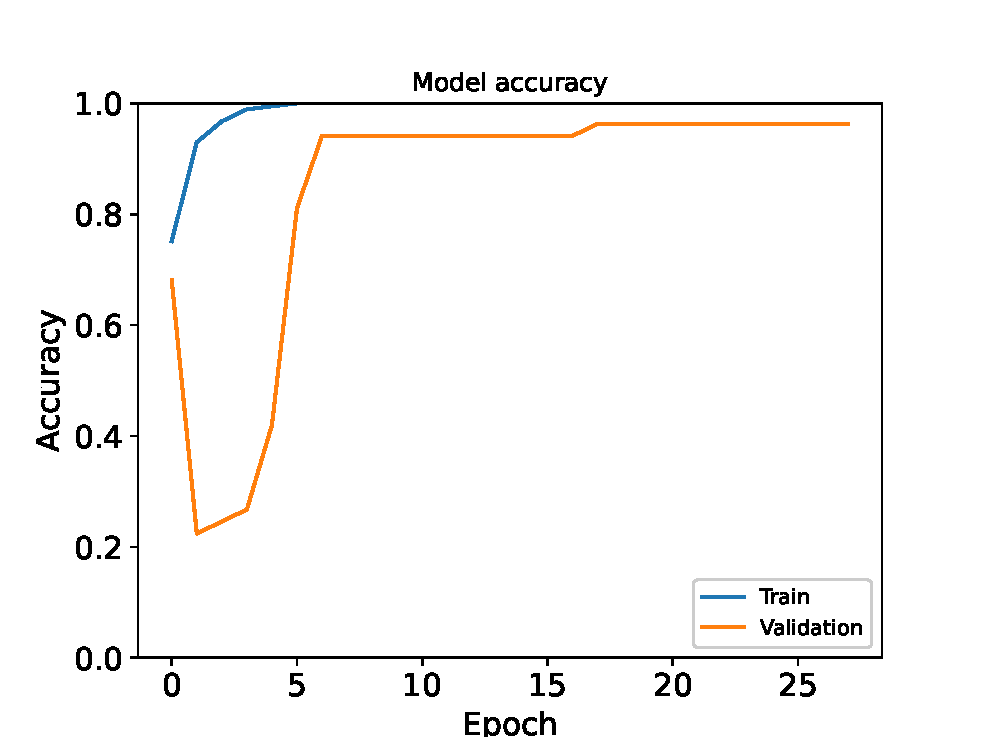
\includegraphics[width=\textwidth]{./fig/model4/accuracy4.eps}
        \caption{Model-4 accuracy}
        \label{fig:model4_accuracy}
    \end{minipage}
    \begin{minipage}{0.45\textwidth}
        \centering
        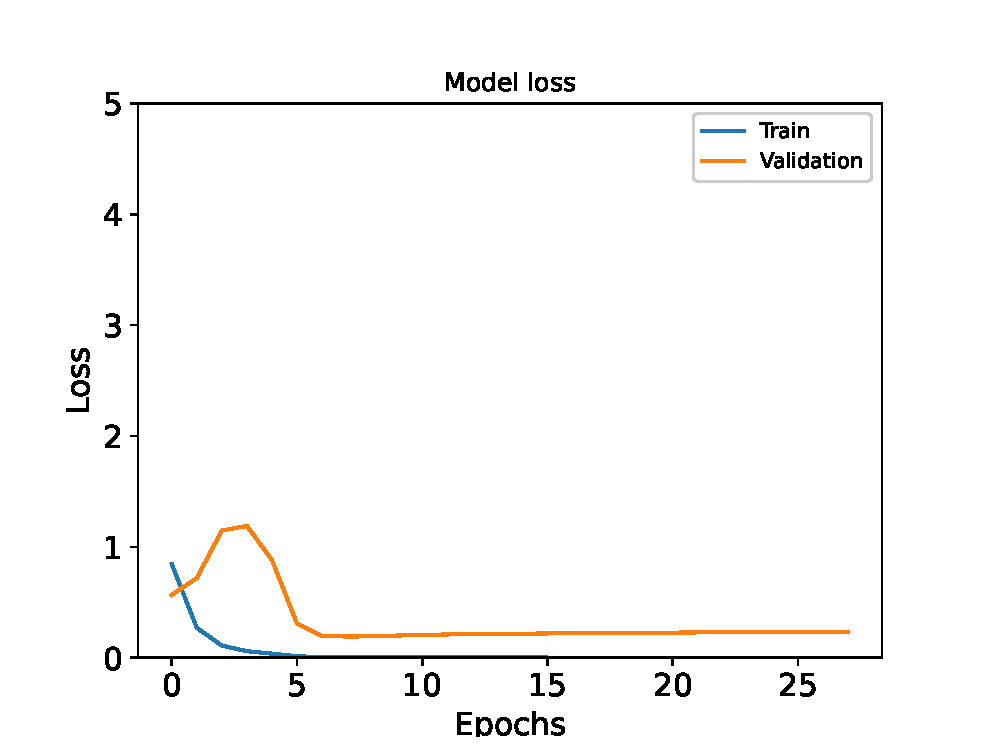
\includegraphics[width=\textwidth]{./fig/model4/loss4.eps}
        \caption{Model-4 loss}
        \label{fig:model4_loss}
    \end{minipage}
\end{figure}

观察训练准确度和损失随步长的变化可以发现,模型的性能有惊人的明显提升。其训练和验证准确度都已经逼近于1,验证集的损失也下降至0.2左右。这说明模型的泛化能力较强,可以很好地适应新的数据。






